\documentclass[12pt,a3paper]{article}
\usepackage{tikz}
\usepackage[margin=0.5in]{geometry}
\usepackage{graphicx}
\usetikzlibrary{arrows.meta,positioning,shapes.geometric}

\begin{document}

\section*{Northern Italy Highway Network Topology}

This figure presents the complete topology of the Northern Italy highway network used 
in the ITER-FLOW traffic assignment model. The network comprises:
\begin{itemize}
  \item 93 nodes representing highway junctions, cities, and border crossings
  \item 232 bidirectional arcs representing highway segments
  \item Node categories: Border crossings (blue), tourist attractions (green), 
        high demand areas (orange), and standard junctions (gray)
\end{itemize}

\begin{center}
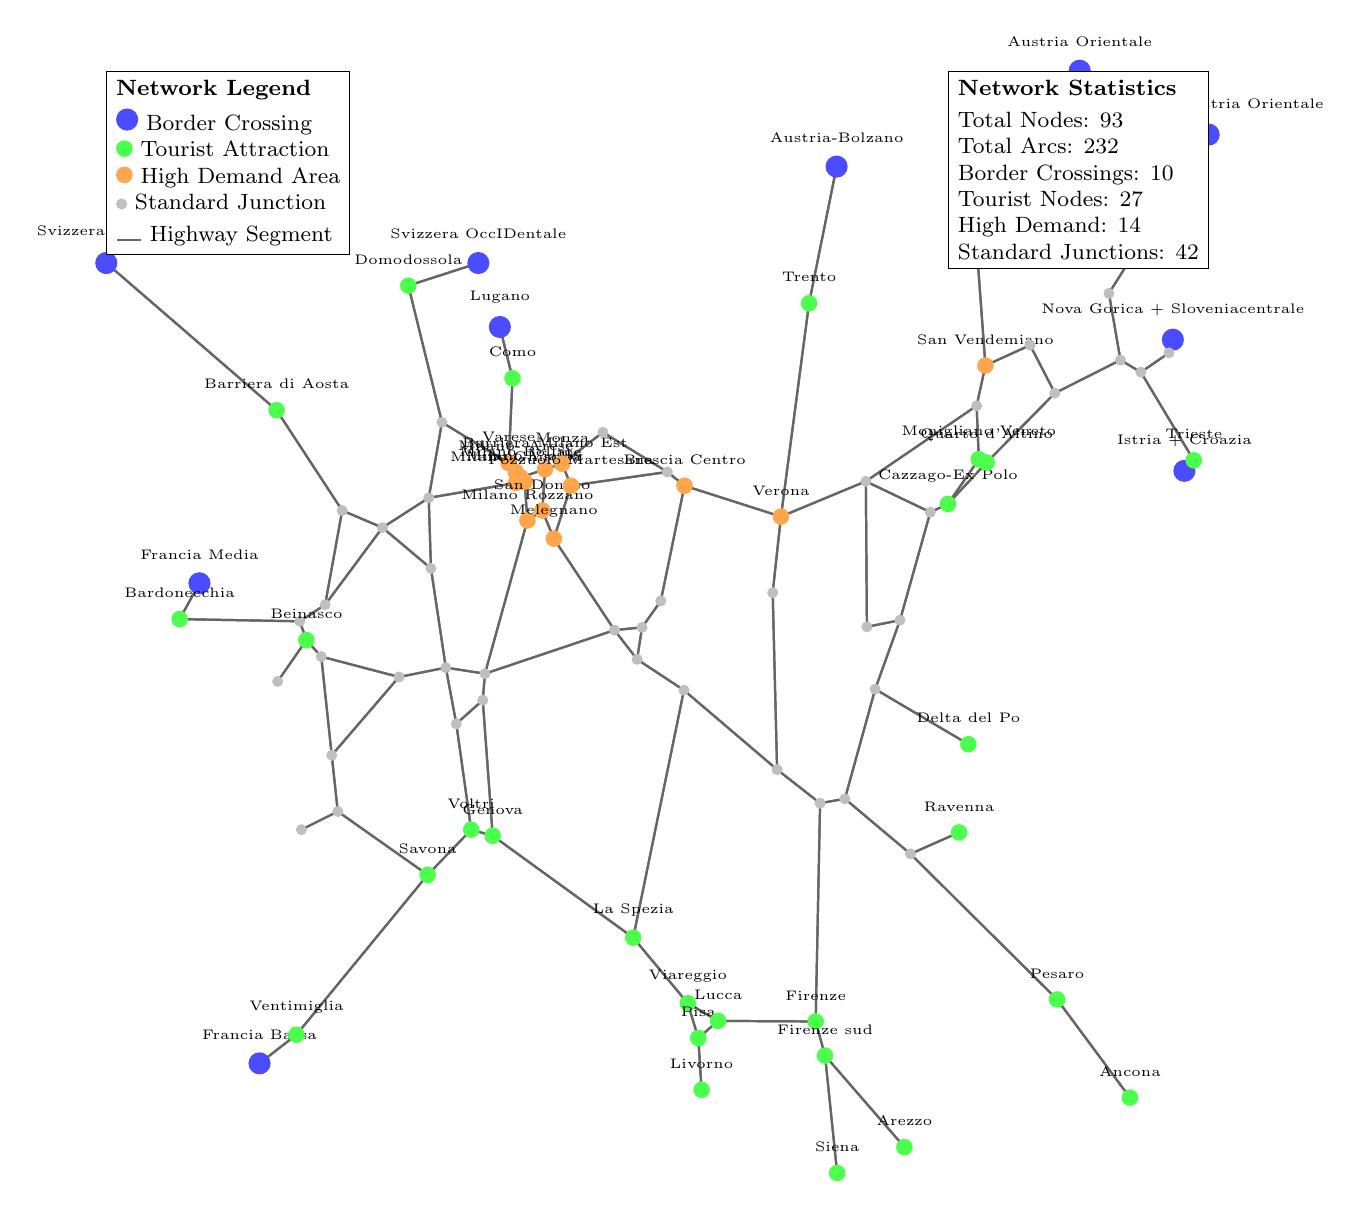
\begin{tikzpicture}[scale=0.7, every node/.style={font=\tiny}]

  % Define node and edge styles
  \tikzstyle{border}=[circle, fill=blue!70, inner sep=2pt, minimum size=8pt]
  \tikzstyle{tourist}=[circle, fill=green!70, inner sep=1.5pt, minimum size=6pt]
  \tikzstyle{highdemand}=[circle, fill=orange!70, inner sep=1.5pt, minimum size=6pt]
  \tikzstyle{normal}=[circle, fill=gray!50, inner sep=1pt, minimum size=4pt]
  \tikzstyle{highway}=[draw=black!60, line width=0.8pt]

  % Highway network arcs
  \draw[highway] (3.09,13.84) -- (4.28,12.02);
  \draw[highway] (4.28,12.02) -- (3.09,13.84);
  \draw[highway] (4.28,12.02) -- (3.97,10.31);
  \draw[highway] (3.97,10.31) -- (4.28,12.02);
  \draw[highway] (4.28,12.02) -- (5.01,11.71);
  \draw[highway] (5.01,11.71) -- (4.28,12.02);
  \draw[highway] (5.01,11.71) -- (3.97,10.31);
  \draw[highway] (3.97,10.31) -- (5.01,11.71);
  \draw[highway] (3.97,10.31) -- (3.51,10.01);
  \draw[highway] (3.51,10.01) -- (3.97,10.31);
  \draw[highway] (3.51,10.01) -- (1.33,10.05);
  \draw[highway] (1.33,10.05) -- (3.51,10.01);
  \draw[highway] (3.51,10.01) -- (3.63,9.67);
  \draw[highway] (3.63,9.67) -- (3.51,10.01);
  \draw[highway] (3.63,9.67) -- (3.90,9.37);
  \draw[highway] (3.90,9.37) -- (3.63,9.67);
  \draw[highway] (3.63,9.67) -- (3.11,8.92);
  \draw[highway] (3.11,8.92) -- (3.63,9.67);
  \draw[highway] (3.90,9.37) -- (4.09,7.58);
  \draw[highway] (4.09,7.58) -- (3.90,9.37);
  \draw[highway] (3.90,9.37) -- (5.31,9.00);
  \draw[highway] (4.09,7.58) -- (4.20,6.56);
  \draw[highway] (4.09,7.58) -- (5.31,9.00);
  \draw[highway] (4.20,6.56) -- (3.54,6.23);
  \draw[highway] (4.20,6.56) -- (5.83,5.41);
  \draw[highway] (5.83,5.41) -- (3.45,2.51);
  \draw[highway] (5.83,5.41) -- (6.62,6.23);
  \draw[highway] (6.62,6.23) -- (6.35,8.15);
  \draw[highway] (6.35,8.15) -- (6.16,9.17);
  \draw[highway] (6.16,9.17) -- (5.31,9.00);
  \draw[highway] (6.16,9.17) -- (5.89,10.97);
  \draw[highway] (5.89,10.97) -- (5.01,11.71);
  \draw[highway] (5.01,11.71) -- (5.85,12.25);
  \draw[highway] (5.89,10.97) -- (5.85,12.25);
  \draw[highway] (5.85,12.25) -- (6.09,13.62);
  \draw[highway] (6.09,13.62) -- (5.48,16.10);
  \draw[highway] (5.85,12.25) -- (7.43,12.52);
  \draw[highway] (6.09,13.62) -- (7.30,12.88);
  \draw[highway] (7.30,12.88) -- (7.37,14.42);
  \draw[highway] (7.30,12.88) -- (7.43,12.72);
  \draw[highway] (7.43,12.72) -- (7.52,12.62);
  \draw[highway] (7.43,12.72) -- (7.43,12.52);
  \draw[highway] (7.52,12.62) -- (7.59,12.54);
  \draw[highway] (7.59,12.54) -- (7.64,11.84);
  \draw[highway] (7.64,11.84) -- (6.87,9.06);
  \draw[highway] (6.87,9.06) -- (6.16,9.17);
  \draw[highway] (6.87,9.06) -- (6.83,8.58);
  \draw[highway] (6.83,8.58) -- (6.35,8.15);
  \draw[highway] (6.83,8.58) -- (7.01,6.12);
  \draw[highway] (7.01,6.12) -- (6.62,6.23);
  \draw[highway] (7.52,12.62) -- (7.96,12.77);
  \draw[highway] (7.96,12.77) -- (7.91,12.02);
  \draw[highway] (7.91,12.02) -- (7.64,11.84);
  \draw[highway] (7.96,12.77) -- (8.27,12.87);
  \draw[highway] (8.27,12.87) -- (8.43,12.47);
  \draw[highway] (8.43,12.47) -- (8.12,11.51);
  \draw[highway] (7.91,12.02) -- (8.12,11.51);
  \draw[highway] (8.12,11.51) -- (9.22,9.85);
  \draw[highway] (9.22,9.85) -- (6.87,9.06);
  \draw[highway] (9.22,9.85) -- (9.63,9.32);
  \draw[highway] (9.22,9.85) -- (9.72,9.90);
  \draw[highway] (9.72,9.90) -- (9.63,9.32);
  \draw[highway] (8.27,12.87) -- (9.01,13.44);
  \draw[highway] (9.01,13.44) -- (10.18,12.72);
  \draw[highway] (10.18,12.72) -- (8.43,12.47);
  \draw[highway] (10.18,12.72) -- (10.49,12.47);
  \draw[highway] (10.49,12.47) -- (10.06,10.38);
  \draw[highway] (10.06,10.38) -- (9.72,9.90);
  \draw[highway] (9.63,9.32) -- (10.48,8.76);
  \draw[highway] (9.56,4.27) -- (10.48,8.76);
  \draw[highway] (7.01,6.12) -- (9.56,4.27);
  \draw[highway] (10.55,3.08) -- (9.56,4.27);
  \draw[highway] (12.17,7.32) -- (10.48,8.76);
  \draw[highway] (12.09,10.53) -- (12.17,7.32);
  \draw[highway] (12.24,11.91) -- (12.09,10.53);
  \draw[highway] (12.75,15.78) -- (12.24,11.91);
  \draw[highway] (10.49,12.47) -- (12.24,11.91);
  \draw[highway] (13.78,12.55) -- (12.24,11.91);
  \draw[highway] (11.10,2.76) -- (10.55,3.08);
  \draw[highway] (10.74,2.45) -- (10.55,3.08);
  \draw[highway] (10.80,1.51) -- (10.74,2.45);
  \draw[highway] (11.10,2.76) -- (10.74,2.45);
  \draw[highway] (12.87,2.75) -- (11.10,2.76);
  \draw[highway] (13.04,2.13) -- (12.87,2.75);
  \draw[highway] (13.26,0.00) -- (13.04,2.13);
  \draw[highway] (14.48,0.47) -- (13.04,2.13);
  \draw[highway] (12.95,6.71) -- (12.87,2.75);
  \draw[highway] (12.17,7.32) -- (12.95,6.71);
  \draw[highway] (13.40,6.79) -- (12.95,6.71);
  \draw[highway] (14.59,5.79) -- (13.40,6.79);
  \draw[highway] (13.95,8.78) -- (13.40,6.79);
  \draw[highway] (15.64,7.78) -- (13.95,8.78);
  \draw[highway] (14.40,10.03) -- (13.95,8.78);
  \draw[highway] (13.80,9.91) -- (14.40,10.03);
  \draw[highway] (13.78,12.55) -- (13.80,9.91);
  \draw[highway] (14.95,11.99) -- (13.78,12.55);
  \draw[highway] (15.79,13.92) -- (13.78,12.55);
  \draw[highway] (14.40,10.03) -- (14.95,11.99);
  \draw[highway] (15.27,12.14) -- (14.95,11.99);
  \draw[highway] (15.97,12.89) -- (15.27,12.14);
  \draw[highway] (15.83,12.95) -- (15.97,12.89);
  \draw[highway] (17.21,14.15) -- (15.97,12.89);
  \draw[highway] (15.27,12.14) -- (15.83,12.95);
  \draw[highway] (15.83,12.95) -- (15.79,13.92);
  \draw[highway] (15.95,14.65) -- (15.79,13.92);
  \draw[highway] (15.81,16.55) -- (15.95,14.65);
  \draw[highway] (15.95,14.65) -- (16.76,15.02);
  \draw[highway] (16.76,15.02) -- (17.21,14.15);
  \draw[highway] (17.21,14.15) -- (18.40,14.75);
  \draw[highway] (18.40,14.75) -- (18.19,15.96);
  \draw[highway] (18.40,14.75) -- (18.77,14.53);
  \draw[highway] (18.77,14.53) -- (19.28,14.88);
  \draw[highway] (18.77,14.53) -- (19.73,12.93);
  \draw[highway] (14.59,5.79) -- (15.47,6.18);
  \draw[highway] (17.25,3.15) -- (14.59,5.79);
  \draw[highway] (18.57,1.37) -- (17.25,3.15);
  \draw[highway] (0.00,16.51) -- (3.09,13.84);
  \draw[highway] (3.09,13.84) -- (0.00,16.51);
  \draw[highway] (1.69,10.70) -- (1.33,10.05);
  \draw[highway] (1.33,10.05) -- (1.69,10.70);
  \draw[highway] (2.78,1.99) -- (3.45,2.51);
  \draw[highway] (3.45,2.51) -- (2.78,1.99);
  \draw[highway] (6.75,16.51) -- (5.48,16.10);
  \draw[highway] (5.48,16.10) -- (6.75,16.51);
  \draw[highway] (7.14,15.35) -- (7.37,14.42);
  \draw[highway] (7.37,14.42) -- (7.14,15.35);
  \draw[highway] (13.25,18.26) -- (12.75,15.78);
  \draw[highway] (12.75,15.78) -- (13.25,18.26);
  \draw[highway] (17.66,20.00) -- (15.81,16.55);
  \draw[highway] (15.81,16.55) -- (17.66,20.00);
  \draw[highway] (20.00,18.84) -- (18.19,15.96);
  \draw[highway] (18.19,15.96) -- (20.00,18.84);
  \draw[highway] (19.35,15.12) -- (19.28,14.88);
  \draw[highway] (19.28,14.88) -- (19.35,15.12);
  \draw[highway] (19.56,12.74) -- (19.73,12.93);
  \draw[highway] (19.73,12.93) -- (19.56,12.74);
  \draw[highway] (5.31,9.00) -- (3.90,9.37);
  \draw[highway] (4.20,6.56) -- (4.09,7.58);
  \draw[highway] (5.31,9.00) -- (4.09,7.58);
  \draw[highway] (3.54,6.23) -- (4.20,6.56);
  \draw[highway] (5.83,5.41) -- (4.20,6.56);
  \draw[highway] (3.45,2.51) -- (5.83,5.41);
  \draw[highway] (6.62,6.23) -- (5.83,5.41);
  \draw[highway] (6.35,8.15) -- (6.62,6.23);
  \draw[highway] (6.16,9.17) -- (6.35,8.15);
  \draw[highway] (5.31,9.00) -- (6.16,9.17);
  \draw[highway] (5.89,10.97) -- (6.16,9.17);
  \draw[highway] (5.01,11.71) -- (5.89,10.97);
  \draw[highway] (5.85,12.25) -- (5.01,11.71);
  \draw[highway] (5.85,12.25) -- (5.89,10.97);
  \draw[highway] (6.09,13.62) -- (5.85,12.25);
  \draw[highway] (5.48,16.10) -- (6.09,13.62);
  \draw[highway] (7.43,12.52) -- (5.85,12.25);
  \draw[highway] (7.30,12.88) -- (6.09,13.62);
  \draw[highway] (7.37,14.42) -- (7.30,12.88);
  \draw[highway] (7.43,12.72) -- (7.30,12.88);
  \draw[highway] (7.52,12.62) -- (7.43,12.72);
  \draw[highway] (7.43,12.52) -- (7.43,12.72);
  \draw[highway] (7.59,12.54) -- (7.52,12.62);
  \draw[highway] (7.64,11.84) -- (7.59,12.54);
  \draw[highway] (6.87,9.06) -- (7.64,11.84);
  \draw[highway] (6.16,9.17) -- (6.87,9.06);
  \draw[highway] (6.83,8.58) -- (6.87,9.06);
  \draw[highway] (6.35,8.15) -- (6.83,8.58);
  \draw[highway] (7.01,6.12) -- (6.83,8.58);
  \draw[highway] (6.62,6.23) -- (7.01,6.12);
  \draw[highway] (7.96,12.77) -- (7.52,12.62);
  \draw[highway] (7.91,12.02) -- (7.96,12.77);
  \draw[highway] (7.64,11.84) -- (7.91,12.02);
  \draw[highway] (8.27,12.87) -- (7.96,12.77);
  \draw[highway] (8.43,12.47) -- (8.27,12.87);
  \draw[highway] (8.12,11.51) -- (8.43,12.47);
  \draw[highway] (8.12,11.51) -- (7.91,12.02);
  \draw[highway] (9.22,9.85) -- (8.12,11.51);
  \draw[highway] (6.87,9.06) -- (9.22,9.85);
  \draw[highway] (9.63,9.32) -- (9.22,9.85);
  \draw[highway] (9.72,9.90) -- (9.22,9.85);
  \draw[highway] (9.63,9.32) -- (9.72,9.90);
  \draw[highway] (9.01,13.44) -- (8.27,12.87);
  \draw[highway] (10.18,12.72) -- (9.01,13.44);
  \draw[highway] (8.43,12.47) -- (10.18,12.72);
  \draw[highway] (10.49,12.47) -- (10.18,12.72);
  \draw[highway] (10.06,10.38) -- (10.49,12.47);
  \draw[highway] (9.72,9.90) -- (10.06,10.38);
  \draw[highway] (10.48,8.76) -- (9.63,9.32);
  \draw[highway] (10.48,8.76) -- (9.56,4.27);
  \draw[highway] (9.56,4.27) -- (7.01,6.12);
  \draw[highway] (9.56,4.27) -- (10.55,3.08);
  \draw[highway] (10.48,8.76) -- (12.17,7.32);
  \draw[highway] (12.17,7.32) -- (12.09,10.53);
  \draw[highway] (12.09,10.53) -- (12.24,11.91);
  \draw[highway] (12.24,11.91) -- (12.75,15.78);
  \draw[highway] (12.24,11.91) -- (10.49,12.47);
  \draw[highway] (12.24,11.91) -- (13.78,12.55);
  \draw[highway] (10.55,3.08) -- (11.10,2.76);
  \draw[highway] (10.55,3.08) -- (10.74,2.45);
  \draw[highway] (10.74,2.45) -- (10.80,1.51);
  \draw[highway] (10.74,2.45) -- (11.10,2.76);
  \draw[highway] (11.10,2.76) -- (12.87,2.75);
  \draw[highway] (12.87,2.75) -- (13.04,2.13);
  \draw[highway] (13.04,2.13) -- (13.26,0.00);
  \draw[highway] (13.04,2.13) -- (14.48,0.47);
  \draw[highway] (12.87,2.75) -- (12.95,6.71);
  \draw[highway] (12.95,6.71) -- (12.17,7.32);
  \draw[highway] (12.95,6.71) -- (13.40,6.79);
  \draw[highway] (13.40,6.79) -- (14.59,5.79);
  \draw[highway] (13.40,6.79) -- (13.95,8.78);
  \draw[highway] (13.95,8.78) -- (15.64,7.78);
  \draw[highway] (13.95,8.78) -- (14.40,10.03);
  \draw[highway] (14.40,10.03) -- (13.80,9.91);
  \draw[highway] (13.80,9.91) -- (13.78,12.55);
  \draw[highway] (13.78,12.55) -- (14.95,11.99);
  \draw[highway] (13.78,12.55) -- (15.79,13.92);
  \draw[highway] (14.95,11.99) -- (14.40,10.03);
  \draw[highway] (14.95,11.99) -- (15.27,12.14);
  \draw[highway] (15.27,12.14) -- (15.97,12.89);
  \draw[highway] (15.97,12.89) -- (15.83,12.95);
  \draw[highway] (15.97,12.89) -- (17.21,14.15);
  \draw[highway] (15.83,12.95) -- (15.27,12.14);
  \draw[highway] (15.79,13.92) -- (15.83,12.95);
  \draw[highway] (15.79,13.92) -- (15.95,14.65);
  \draw[highway] (15.95,14.65) -- (15.81,16.55);
  \draw[highway] (16.76,15.02) -- (15.95,14.65);
  \draw[highway] (17.21,14.15) -- (16.76,15.02);
  \draw[highway] (18.40,14.75) -- (17.21,14.15);
  \draw[highway] (18.19,15.96) -- (18.40,14.75);
  \draw[highway] (18.77,14.53) -- (18.40,14.75);
  \draw[highway] (19.28,14.88) -- (18.77,14.53);
  \draw[highway] (19.73,12.93) -- (18.77,14.53);
  \draw[highway] (15.47,6.18) -- (14.59,5.79);
  \draw[highway] (14.59,5.79) -- (17.25,3.15);
  \draw[highway] (17.25,3.15) -- (18.57,1.37);

  % Total arcs drawn: 232

  % Network nodes
  \node[border] (chf) at (0.00,16.51) {};
  \node[above=1pt of chf, font=\tiny] {Svizzera/Francia};
  \node[tourist] (1) at (3.09,13.84) {};
  \node[above=1pt of 1, font=\tiny] {Barriera di Aosta};
  \node[normal] (2) at (4.28,12.02) {};
  \node[normal] (3) at (3.97,10.31) {};
  \node[normal] (4) at (3.51,10.01) {};
  \node[border] (fr1) at (1.69,10.70) {};
  \node[above=1pt of fr1, font=\tiny] {Francia Media};
  \node[tourist] (5) at (1.33,10.05) {};
  \node[above=1pt of 5, font=\tiny] {Bardonecchia};
  \node[tourist] (6) at (3.63,9.67) {};
  \node[above=1pt of 6, font=\tiny] {Beinasco};
  \node[normal] (7) at (3.11,8.92) {};
  \node[normal] (8) at (3.90,9.37) {};
  \node[normal] (9) at (4.20,6.56) {};
  \node[normal] (10) at (3.54,6.23) {};
  \node[tourist] (11) at (5.83,5.41) {};
  \node[above=1pt of 11, font=\tiny] {Savona};
  \node[border] (fr2) at (2.78,1.99) {};
  \node[above=1pt of fr2, font=\tiny] {Francia Bassa};
  \node[tourist] (12) at (3.45,2.51) {};
  \node[above=1pt of 12, font=\tiny] {Ventimiglia};
  \node[normal] (13) at (5.01,11.71) {};
  \node[normal] (14) at (5.31,9.00) {};
  \node[normal] (15) at (4.09,7.58) {};
  \node[normal] (16) at (5.85,12.25) {};
  \node[normal] (17) at (5.89,10.97) {};
  \node[normal] (18) at (6.16,9.17) {};
  \node[normal] (19) at (6.35,8.15) {};
  \node[tourist] (20) at (6.62,6.23) {};
  \node[above=1pt of 20, font=\tiny] {Voltri};
  \node[border] (ch1) at (6.75,16.51) {};
  \node[above=1pt of ch1, font=\tiny] {Svizzera OccIDentale};
  \node[tourist] (21) at (5.48,16.10) {};
  \node[above=1pt of 21, font=\tiny] {Domodossola};
  \node[normal] (22) at (6.09,13.62) {};
  \node[border] (ch2) at (7.14,15.35) {};
  \node[above=1pt of ch2, font=\tiny] {Lugano};
  \node[tourist] (23) at (7.37,14.42) {};
  \node[above=1pt of 23, font=\tiny] {Como};
  \node[highdemand] (24) at (7.30,12.88) {};
  \node[above=1pt of 24, font=\tiny] {Varese};
  \node[highdemand] (25) at (7.43,12.72) {};
  \node[above=1pt of 25, font=\tiny] {Milano- Arese};
  \node[highdemand] (25-b) at (7.52,12.62) {};
  \node[above=1pt of 25-b, font=\tiny] {Milano Bollate};
  \node[highdemand] (25-d) at (7.59,12.54) {};
  \node[above=1pt of 25-d, font=\tiny] {Milano Vialba};
  \node[highdemand] (25-c) at (7.43,12.52) {};
  \node[above=1pt of 25-c, font=\tiny] {Milano Ghisolfa};
  \node[highdemand] (26) at (7.64,11.84) {};
  \node[above=1pt of 26, font=\tiny] {Milano Rozzano};
  \node[normal] (27) at (6.87,9.06) {};
  \node[normal] (28) at (6.83,8.58) {};
  \node[tourist] (29) at (7.01,6.12) {};
  \node[above=1pt of 29, font=\tiny] {Genova};
  \node[highdemand] (30) at (7.96,12.77) {};
  \node[above=1pt of 30, font=\tiny] {Barriera Milano Est};
  \node[highdemand] (31) at (7.91,12.02) {};
  \node[above=1pt of 31, font=\tiny] {San Donato};
  \node[highdemand] (32) at (8.27,12.87) {};
  \node[above=1pt of 32, font=\tiny] {Monza};
  \node[highdemand] (33) at (8.43,12.47) {};
  \node[above=1pt of 33, font=\tiny] {Pozzuolo Martesana};
  \node[highdemand] (34) at (8.12,11.51) {};
  \node[above=1pt of 34, font=\tiny] {Melegnano};
  \node[normal] (35) at (9.22,9.85) {};
  \node[normal] (36) at (9.72,9.90) {};
  \node[normal] (37) at (9.63,9.32) {};
  \node[tourist] (38) at (9.56,4.27) {};
  \node[above=1pt of 38, font=\tiny] {La Spezia};
  \node[normal] (39) at (9.01,13.44) {};
  \node[normal] (40) at (10.18,12.72) {};
  \node[highdemand] (41) at (10.49,12.47) {};
  \node[above=1pt of 41, font=\tiny] {Brescia Centro};
  \node[normal] (42) at (10.06,10.38) {};
  \node[normal] (43) at (10.48,8.76) {};
  \node[border] (au) at (13.25,18.26) {};
  \node[above=1pt of au, font=\tiny] {Austria-Bolzano};
  \node[tourist] (44) at (12.75,15.78) {};
  \node[above=1pt of 44, font=\tiny] {Trento};
  \node[highdemand] (45) at (12.24,11.91) {};
  \node[above=1pt of 45, font=\tiny] {Verona};
  \node[normal] (46) at (12.09,10.53) {};
  \node[normal] (47) at (12.17,7.32) {};
  \node[tourist] (48) at (10.55,3.08) {};
  \node[above=1pt of 48, font=\tiny] {Viareggio};
  \node[tourist] (49) at (10.74,2.45) {};
  \node[above=1pt of 49, font=\tiny] {Pisa};
  \node[tourist] (50) at (11.10,2.76) {};
  \node[above=1pt of 50, font=\tiny] {Lucca};
  \node[tourist] (51) at (10.80,1.51) {};
  \node[above=1pt of 51, font=\tiny] {Livorno};
  \node[tourist] (52) at (12.87,2.75) {};
  \node[above=1pt of 52, font=\tiny] {Firenze};
  \node[tourist] (53) at (13.04,2.13) {};
  \node[above=1pt of 53, font=\tiny] {Firenze sud};
  \node[tourist] (54) at (13.26,0.00) {};
  \node[above=1pt of 54, font=\tiny] {Siena};
  \node[tourist] (55) at (14.48,0.47) {};
  \node[above=1pt of 55, font=\tiny] {Arezzo};
  \node[normal] (56) at (12.95,6.71) {};
  \node[normal] (57) at (13.78,12.55) {};
  \node[border] (au2) at (17.66,20.00) {};
  \node[above=1pt of au2, font=\tiny] {Austria Orientale};
  \node[normal] (58) at (15.81,16.55) {};
  \node[normal] (59) at (15.79,13.92) {};
  \node[normal] (60) at (14.95,11.99) {};
  \node[normal] (61) at (13.80,9.91) {};
  \node[normal] (62) at (14.40,10.03) {};
  \node[normal] (63) at (13.95,8.78) {};
  \node[normal] (64) at (13.40,6.79) {};
  \node[normal] (65) at (14.59,5.79) {};
  \node[tourist] (66) at (17.25,3.15) {};
  \node[above=1pt of 66, font=\tiny] {Pesaro};
  \node[tourist] (67) at (18.57,1.37) {};
  \node[above=1pt of 67, font=\tiny] {Ancona};
  \node[tourist] (68) at (15.47,6.18) {};
  \node[above=1pt of 68, font=\tiny] {Ravenna};
  \node[tourist] (69) at (15.64,7.78) {};
  \node[above=1pt of 69, font=\tiny] {Delta del Po};
  \node[tourist] (70) at (15.27,12.14) {};
  \node[above=1pt of 70, font=\tiny] {Cazzago-Ex Polo};
  \node[tourist] (71) at (15.83,12.95) {};
  \node[above=1pt of 71, font=\tiny] {Monigliano Veneto};
  \node[tourist] (72) at (15.97,12.89) {};
  \node[above=1pt of 72, font=\tiny] {Quarto d'Altino};
  \node[highdemand] (73) at (15.95,14.65) {};
  \node[above=1pt of 73, font=\tiny] {San Vendemiano};
  \node[normal] (74) at (16.76,15.02) {};
  \node[normal] (75) at (17.21,14.15) {};
  \node[border] (au3) at (20.00,18.84) {};
  \node[above=1pt of au3, font=\tiny] {Villach + Austria Orientale};
  \node[normal] (76) at (18.19,15.96) {};
  \node[normal] (77) at (18.40,14.75) {};
  \node[normal] (78) at (18.77,14.53) {};
  \node[border] (slo1) at (19.35,15.12) {};
  \node[above=1pt of slo1, font=\tiny] {Nova Gorica + Sloveniacentrale};
  \node[normal] (79) at (19.28,14.88) {};
  \node[border] (slo2) at (19.56,12.74) {};
  \node[above=1pt of slo2, font=\tiny] {Istria + Croazia};
  \node[tourist] (80) at (19.73,12.93) {};
  \node[above=1pt of 80, font=\tiny] {Trieste};

  % Node count: Border=10, Tourist=27, HighDemand=14, Normal=42

  % Legend
  \node[anchor=north west, draw=black, fill=white, align=left, font=\footnotesize] at (0, 20) {
    \textbf{Network Legend} \\[2pt]
    \tikz\node[border] {}; Border Crossing \\
    \tikz\node[tourist] {}; Tourist Attraction \\
    \tikz\node[highdemand] {}; High Demand Area \\
    \tikz\node[normal] {}; Standard Junction \\[2pt]
    \tikz\draw[highway] (0,0) -- (0.3,0); Highway Segment
  };

  % Network Statistics
  \node[anchor=north east, draw=black, fill=white, align=left, font=\footnotesize] at (20, 20) {
    \textbf{Network Statistics} \\[2pt]
    Total Nodes: 93 \\
    Total Arcs: 232 \\
    Border Crossings: 10 \\
    Tourist Nodes: 27 \\
    High Demand: 14 \\
    Standard Junctions: 42
  };

\end{tikzpicture}
\end{center}

\clearpage

\section*{Node Directory}

\begin{table}[h]
\centering
\small
\begin{tabular}{llllr}
\hline
\textbf{ID} & \textbf{Name} & \textbf{Category} & \textbf{Coordinates} & \textbf{Population} \\
\hline
1 & Barriera di Aosta & attrazione turistica & (45.74, 7.39) & 123,130 \\
10 & Cuneo & bassa domanda & (44.43, 7.56) & 290,257 \\
11 & Savona & attrazione turistica & (44.29, 8.44) & 267,621 \\
12 & Ventimiglia & attrazione turistica & (43.79, 7.53) & 208,800 \\
13 & Santhià & bassa domanda & (45.37, 8.13) & 88,684 \\
14 & Asti & bassa domanda & (44.91, 8.25) & 218,081 \\
15 & Bra & bassa domanda & (44.66, 7.78) & 325,384 \\
16 & Recetto & bassa domanda & (45.47, 8.45) & 361,904 \\
17 & Vercelli & bassa domanda & (45.25, 8.47) & 88,684 \\
18 & Alessandria & bassa domanda & (44.94, 8.57) & 101,596 \\
19 & Predosa & bassa domanda & (44.76, 8.64) & 101,596 \\
2 & Ivrea & bassa domanda & (45.43, 7.85) & 187,491 \\
20 & Voltri & attrazione turistica & (44.43, 8.75) & 408,814 \\
21 & Domodossola & attrazione turistica & (46.13, 8.31) & 76,881 \\
22 & Comignago & bassa domanda & (45.70, 8.54) & 76,881 \\
23 & Como & attrazione turistica & (45.84, 9.04) & 597,949 \\
24 & Varese & grande domanda & (45.57, 9.01) & 880,257 \\
25 & Milano- Arese & grande domanda & (45.55, 9.06) & 360,607 \\
25-b & Milano Bollate & grande domanda & (45.53, 9.09) & 360,607 \\
25-c & Milano Ghisolfa & grande domanda & (45.51, 9.06) & 360,607 \\
25-d & Milano Vialba & grande domanda & (45.52, 9.12) & 360,607 \\
26 & Milano Rozzano & grande domanda & (45.40, 9.14) & 360,607 \\
27 & Tortona & bassa domanda & (44.92, 8.84) & 101,596 \\
28 & Tortona - 2 & bassa domanda & (44.83, 8.83) & 101,596 \\
29 & Genova & attrazione turistica & (44.41, 8.90) & 408,814 \\
3 & Falchera & bassa domanda & (45.13, 7.73) & 325,384 \\
30 & Barriera Milano Est & grande domanda & (45.56, 9.27) & 360,607 \\
31 & San Donato & grande domanda & (45.43, 9.25) & 360,607 \\
32 & Monza & grande domanda & (45.57, 9.39) & 876,792 \\
33 & Pozzuolo Martesana & grande domanda & (45.50, 9.44) & 360,607 \\
34 & Melegnano & grande domanda & (45.34, 9.33) & 360,607 \\
35 & Piacenza & bassa domanda & (45.05, 9.75) & 95,130 \\
36 & Monticelli d'Ongina & bassa domanda & (45.06, 9.94) & 95,130 \\
37 & Piacenza-Sud & bassa domanda & (44.96, 9.91) & 95,130 \\
38 & La Spezia & attrazione turistica & (44.09, 9.88) & 215,091 \\
39 & Bergamo & bassa domanda & (45.67, 9.67) & 1,110,427 \\
4 & Rivoli & bassa domanda & (45.08, 7.55) & 325,384 \\
40 & Brescia - Ovest & bassa domanda & (45.55, 10.12) & 630,478 \\
41 & Brescia Centro & grande domanda & (45.50, 10.24) & 630,478 \\
42 & Cremona & bassa domanda & (45.14, 10.07) & 352,965 \\
43 & Parma & bassa domanda & (44.86, 10.24) & 454,149 \\
44 & Trento & attrazione turistica & (46.07, 11.11) & 1,082,702 \\
45 & Verona & grande domanda & (45.41, 10.91) & 926,970 \\
46 & Mantova & bassa domanda & (45.17, 10.86) & 407,002 \\
47 & Modena & bassa domanda & (44.62, 10.89) & 706,445 \\
48 & Viareggio & attrazione turistica & (43.89, 10.26) & 186,982 \\
49 & Pisa & attrazione turistica & (43.78, 10.34) & 417,674 \\
5 & Bardonecchia & attrazione turistica & (45.09, 6.71) & 325,384 \\
50 & Lucca & attrazione turistica & (43.83, 10.47) & 381,826 \\
51 & Livorno & attrazione turistica & (43.62, 10.36) & 326,315 \\
52 & Firenze & attrazione turistica & (43.83, 11.16) & 494,393 \\
53 & Firenze sud & attrazione turistica & (43.72, 11.22) & 494,393 \\
54 & Siena & attrazione turistica & (43.36, 11.30) & 259,921 \\
55 & Arezzo & attrazione turistica & (43.44, 11.78) & 333,344 \\
56 & Bologna - Ovest & bassa domanda & (44.51, 11.19) & 508,768 \\
57 & Vicenza & bassa domanda & (45.52, 11.51) & 853,610 \\
58 & Belluno & bassa domanda & (46.21, 12.29) & 99,894 \\
59 & Treviso & bassa domanda & (45.75, 12.28) & 879,388 \\
6 & Beinasco & attrazione turistica & (45.02, 7.60) & 325,384 \\
60 & Padova & bassa domanda & (45.42, 11.96) & 931,607 \\
61 & Badia Polesine & bassa domanda & (45.06, 11.51) & 113,724 \\
62 & Rovigo & bassa domanda & (45.08, 11.74) & 113,724 \\
63 & Ferrara & bassa domanda & (44.87, 11.57) & 339,664 \\
64 & Bologna - Sud & bassa domanda & (44.53, 11.36) & 508,768 \\
65 & Imola & bassa domanda & (44.35, 11.82) & 208,851 \\
66 & Pesaro & attrazione turistica & (43.90, 12.84) & 349,882 \\
67 & Ancona & attrazione turistica & (43.59, 13.35) & 461,629 \\
68 & Ravenna & attrazione turistica & (44.42, 12.16) & 387,229 \\
69 & Delta del Po & attrazione turistica & (44.70, 12.22) & 339,837 \\
7 & Pinerolo & bassa domanda & (44.89, 7.40) & 325,384 \\
70 & Cazzago-Ex Polo & attrazione turistica & (45.45, 12.08) & 208,851 \\
71 & Monigliano Veneto & attrazione turistica & (45.59, 12.29) & 208,851 \\
72 & Quarto d'Altino & attrazione turistica & (45.58, 12.35) & 208,851 \\
73 & San Vendemiano & grande domanda & (45.88, 12.34) & 98,894 \\
74 & Pordenone & bassa domanda & (45.94, 12.65) & 310,763 \\
75 & Portogruaro & bassa domanda & (45.79, 12.83) & 310,763 \\
76 & Udine & bassa domanda & (46.10, 13.20) & 258,572 \\
77 & Palmanova & bassa domanda & (45.90, 13.29) & 258,572 \\
78 & Monfalcone & bassa domanda & (45.86, 13.43) & 69,157 \\
79 & Gorizia & bassa domanda & (45.92, 13.62) & 69,157 \\
8 & Moncalieri & bassa domanda & (44.97, 7.70) & 325,384 \\
80 & Trieste & attrazione turistica & (45.58, 13.80) & 228,396 \\
9 & Carrú & bassa domanda & (44.49, 7.82) & 290,257 \\
au & Austria-Bolzano & ingresso estero & (46.50, 11.30) & 120,000 \\
au2 & Austria Orientale & ingresso estero & (46.80, 13.00) & 150,000 \\
au3 & Villach + Austria Orientale & ingresso estero & (46.60, 13.90) & 60,000 \\
ch1 & Svizzera OccIDentale & ingresso estero & (46.20, 8.80) & 48,000 \\
ch2 & Lugano & ingresso estero & (46.00, 8.95) & 63,000 \\
chf & Svizzera/Francia & ingresso estero & (46.20, 6.20) & 250,000 \\
fr1 & Francia Media & ingresso estero & (45.20, 6.85) & 10,000 \\
fr2 & Francia Bassa & ingresso estero & (43.70, 7.27) & 1,500,000 \\
slo1 & Nova Gorica + Sloveniacentrale & ingresso estero & (45.96, 13.65) & 15,000 \\
slo2 & Istria + Croazia & ingresso estero & (45.55, 13.73) & 25,000 \\
\hline
\end{tabular}
\caption{Complete directory of all 93 nodes in the network.}
\end{table}

\end{document}